%----------------------------------------------------------------------------
\chapter{Jegyzőkönyv}
%----------------------------------------------------------------------------

%----------------------------------------------------------------------------
\section{Első feladat}
%----------------------------------------------------------------------------
\begin{figure}[!ht]
	\centering
	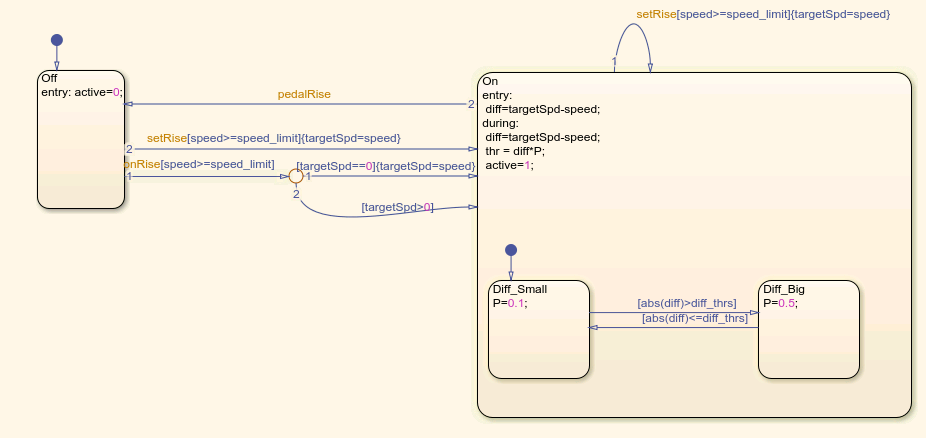
\includegraphics[width=120mm,keepaspectratio]{figures/2m04/f2_chart_2.png}
	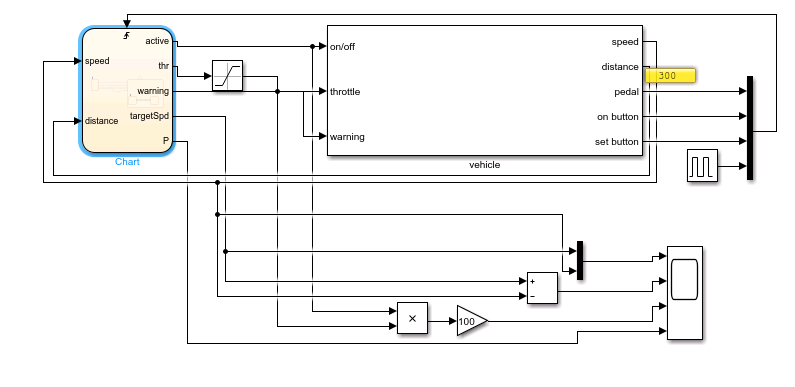
\includegraphics[width=120mm,keepaspectratio]{figures/2m04/f2_model_2.png}
	\caption{Az egyszerű tempomat modellje}
	\label{fig:chart1}
\end{figure}
Az első feladat megoldása során egy tempomatot implementáltam \textit{Stateflow} környezetben. A megvalósított rendszer és a benne található StateChart a \figref{chart1}~ábrán látható. A laboratórium során használt előre megírt Simulink modell az \textit{on/off} bemenetére 0 vagy 1 értéket vár, attól függően, hogy a tempomat aktív-e. Ehhez hasonlóan a \textit{warning} input a harmadik feladatban megvalósítandó jelzés állapotát várja. A kívánt gázpedálállást a \textit{throttle} bemeneten tudjuk egy 0 és 1 közötti értékként megadni a rendszernek. Kimenetként az aktuális sebesség, a jármű előtti akadály távolsága, valamint a nyomógombok és a pedál lenyomásának detektálására szolgáló jelek találhatóak.


A rendszerbe egy $T=0.1s$ periódusidejű pulzusgenerátort tettem, mely felfutó élre triggereli a \textit{StateChart} modellt. Ezen kívül az állapotgép "gázpedál-állás" kimenetét beszaturáltam 0 és 1 közé, hogy ne kaphasson a modell valótlan értéket. A könnyebb fejlesztés érdekében a sebességeket, azok különbségét, a kiadott gázpedál-állást, valamint a használt P erősítést is egy oszcilloszkópon jelenítettem meg, melyet a végleges modellnél kitöröltem.

Az állapotgép az \textit{Off} állapottal indul, ilyenkor a tempomat ki van kapcsolva. Ebből az állapotból az ON vagy a SET gomb megnyomásával lehet a tempomatot bekapcsolt állapotba helyezni. A SET gomb megnyomása esetén -akár bekapcsolt állapotban történő ismételt nyomásra is - a rendszer az aktuális sebességet veszi követendő referencia sebességnek. Az ON gomb esetén, ha már volt tárolt sebesség akkor azt kezdi el használni.

A P-szabályzó figyelembe veszi a különbséget az aktuális és a követendő sebesség között, ez alapján állítja a gyorsítás értékét.

A \figref{scope1}~ábrán ennek az egyszerű modellnek a tesztelése látható, mely során egy kézi gyorsítás után a tempomatot bekapcsoltuk, az pedig követte a referenciasebességet. Mivel ez a rendszer első bekapcsolása volt, a kis hibajel miatt a a P értéke is kicsi maradt. 

\begin{figure}[!ht]
\centering
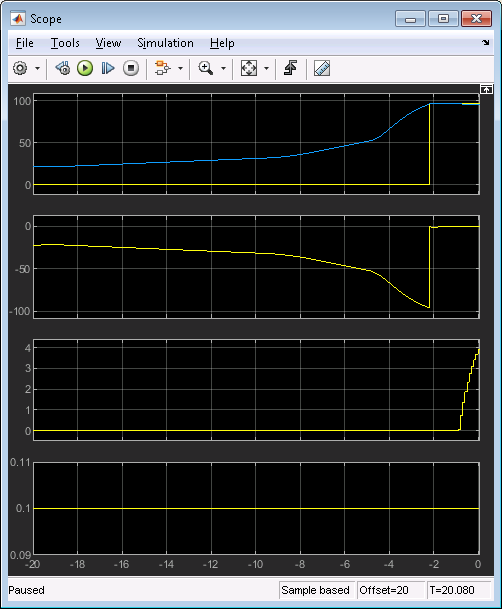
\includegraphics[width=110mm,keepaspectratio]{figures/2m04/f2_scope_2.png}
\caption{Az egyszerű tempomat tesztelése}
\label{fig:scope1}
\end{figure}

\newpage
%----------------------------------------------------------------------------
\section{Második feladat}
%----------------------------------------------------------------------------
\begin{figure}[!ht]
	\centering
	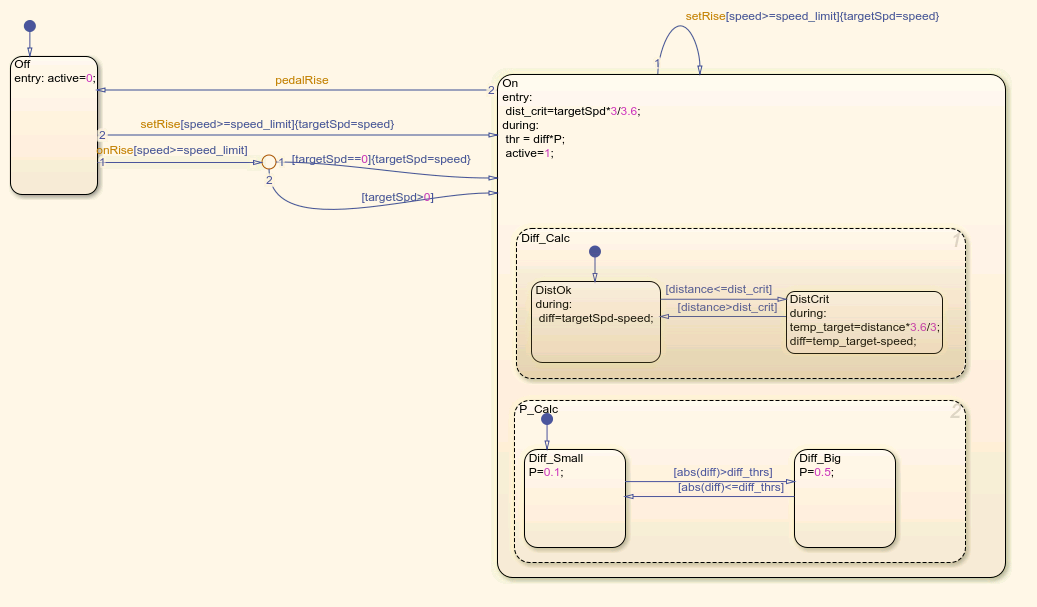
\includegraphics[width=\textwidth,keepaspectratio]{figures/2m04/f2_chart_3.png}
%	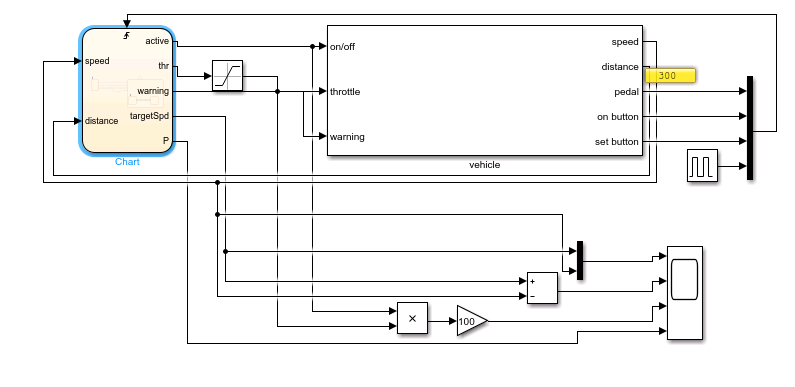
\includegraphics[width=120mm,keepaspectratio]{figures/2m04/f2_model_2.png}
	\caption{Az adaptív tempomat állapotgépe}
	\label{fig:chart2}
\end{figure}

Az adaptív tempomat megvalósítása során a távolságérzékelőből jövő \textit{distance} jelet kellett felhasználni. A beállított referencia sebesség alapján számolható egy kritikus úthossz (a modellben \textit{dist\_crit} nevű változó), mely megadja, hogy az adott sebességgel hány métert tesz meg a jármű a feladatkiírásban szereplő 3 másodperc alatt. A \figref{chart2}~ábrán látható a kibővített állapotgép, mely a \textit{DistOK} állapotban marad, egészen addig, amíg a kritikus úthossz alá nem csökken a \textit{distance} jel. Ekkor a \textit{DistCrit} állapotban a rendszer egy új refrencia sebességet számol a mért távolság alapján, hogy az adaptívan követni tudja a jármű előtti akadályt, például egy másik járművet. Mivel a tempomat bekapcsolt állapota mellett mind a távolság, mind a P erősítés számolását meg kell valósítani, így azokat \textit{AND} kompozícióval valósítottam meg.

\begin{figure}[!ht]
	\centering
	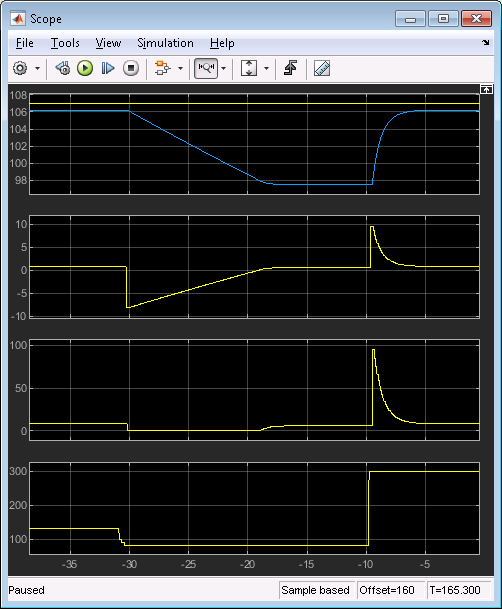
\includegraphics[width=120mm,keepaspectratio]{figures/2m04/f2_scope_3.png}
	\caption{Az adaptív tempomat tesztelése}
	\label{fig:scope2}
\end{figure}



A modell tesztelésére szolgáló mérés a \figref{scope2}~ábrán látható. A kék jel az autó tényleges sebessége, a sárga jelek sorban a sofőr által beállított referencia sebesség, előző kettő különbsége, a kiadott gázpedálállás jel \%-os formában, valamint a távolságérzékelőből jövő jel. Jól látszik, hogy a mérés szüneteltetését előtt kb. \textit{30} másodperccel kritikusan közel jött egy akadály a jármű előtt, ezért a tempomat azonnal elvette a pedálnyomást. Nagyjából \textit{-19s} környékén az autó annyira visszalassult, hogy a követendő távolság tartásához ismét növelni kell a gázpedálnyomás értékét, melyet a rendszer meg is tesz. A mérés vége előtt \textit{10} másodperccel az akadály eltűnt a jármű előtt, így az visszaáll az eredetileg beállított referencia sebesség követésére.

A mérés elején és végén jól látható a P-szabályzó hátránya, a beállított sebességet konstans leköveti, ám a maradandó hiba miatt azt sosem éri el.

\newpage
%----------------------------------------------------------------------------
\section{Harmadik feladat}
%----------------------------------------------------------------------------
A gyorsan érkező akadály jelzésének a tempomattól függetlenül kell működnie, így a \figref{chart3}~ábrán látható módon ismét az \textit{AND} kompozíciót használtam. A jármű és az előtte lévő akadály sebességkülönbségének számításához ismerni kell az előző mintavételi pillanatbani távolságot, valamint a két mintavétel között eltelt időt. A \textit{warning} jel \textbf{1} értéket ad, ha ezen sebességkülönbség egy előre beállított küszöbérték felett van, különben pedig \textbf{0}-t.
\begin{equation}
	\Delta v=\frac{dist_{current}-dist_{prev}}{t_{current}-t_{prev}}\label{dv}
\end{equation}
A \figref{warning}~ábrán a bal oldali képen a bekapcsolt tempomattal történő sebességkövetés, a jobb oldalin pedig a kikapcsolt tempomattal történő jelzés látható.

Habár a jelzés láthatóan működik, a modell bármilyen akadály közeledetével be fog jelezni, mivel a kezelőfelületen a lépték 3 méter, a mintavételi idő pedig 0,1s, ez pedig a beállított $10 \frac{m}{s}$-os küszöbérték háromszorosa. A valós szimuláció érdekében a tempomat fejlesztéséhez érdemes lehet ezen jelet megszűrni, hogy az ugrásszerű változásra ne jelezzen be a rendszer, csak a ténylegesen nagy sebességkülönbségre.

\begin{figure}[!ht]
	\centering
	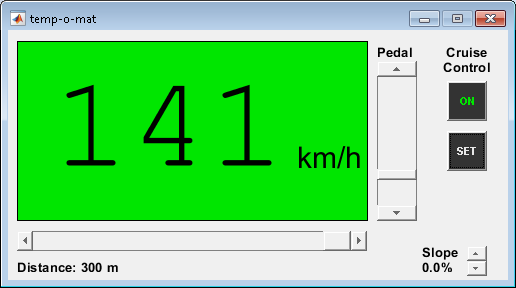
\includegraphics[width=70mm,keepaspectratio]{figures/2m04/f2_tempomat_1.png}	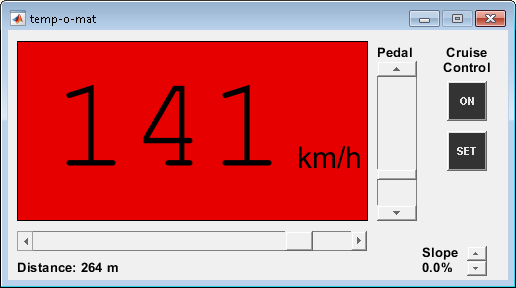
\includegraphics[width=70mm,keepaspectratio]{figures/2m04/f2_tempomat_2.png}
	\caption{A warning jelzés működése kikapcsolt tempomat mellett}
	\label{fig:warning}
\end{figure}


\begin{figure}[!ht]
	\centering
	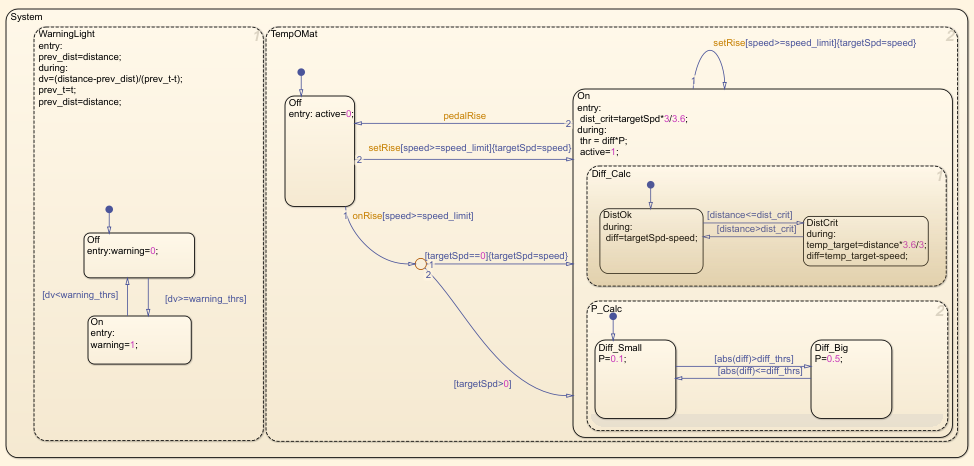
\includegraphics[width=\textwidth,keepaspectratio]{figures/2m04/f2_chart_4.png}
	%	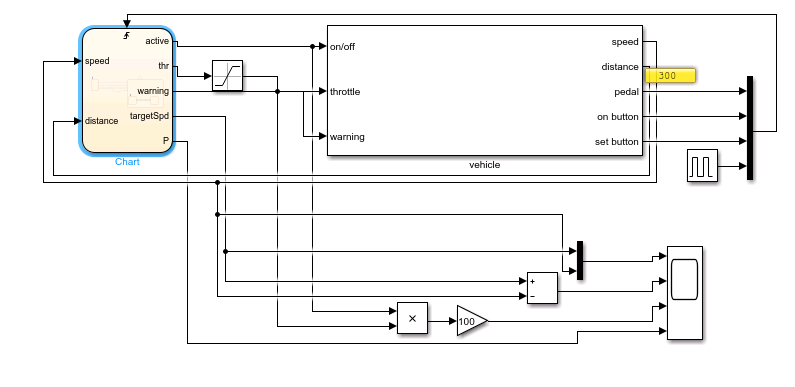
\includegraphics[width=120mm,keepaspectratio]{figures/2m04/f2_model_2.png}
	\caption{Az adaptív tempomat és figyelmeztető jelzés állapotgépe}
	\label{fig:chart3}
\end{figure}

A \figref{model3}~ábrán a letisztított végleges modell, a \figref{variables}~ábrán pedig a \textit{StateChart} modellben használt változók láthatóak. A fejlesztés során használt küszöbértékekhez konstansokat állítottam be, hogy azok könnyen változtathatóak legyenek akár egy másik fajta specifikáció számára is.


\begin{figure}[!ht]
\centering
%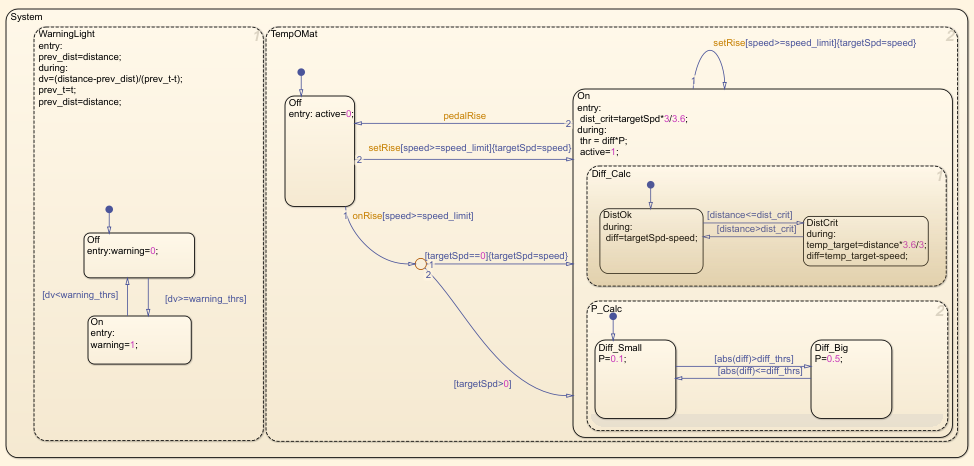
\includegraphics[width=\textwidth,keepaspectratio]{figures/2m04/f2_chart_4.png}
	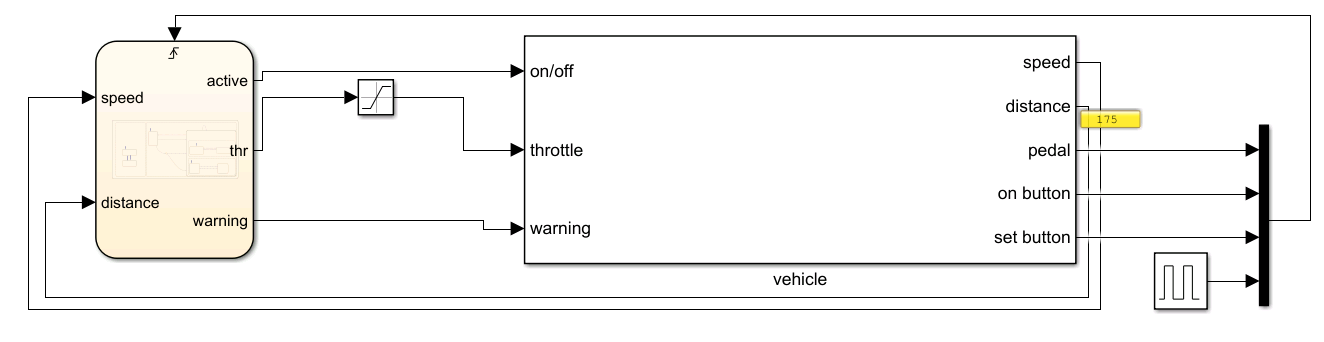
\includegraphics[width=120mm,keepaspectratio]{figures/2m04/f2_model_4.png}
\caption{A végleges modell}
\label{fig:model3}
\end{figure}

\begin{figure}[!ht]
	\centering
	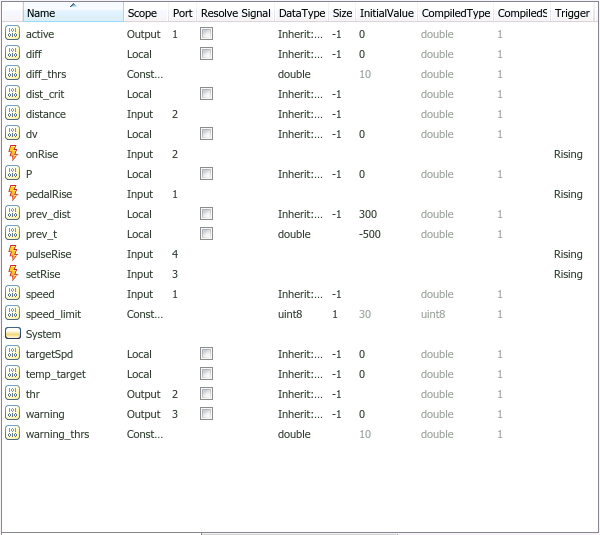
\includegraphics[width=120mm,keepaspectratio]{figures/2m04/variables.png}
	\caption{A végleges modell}
	\label{fig:variables}
\end{figure}